% command to make sure colorboxes don't create whitespace between code lines
\fboxsep=.6pt

% default settings for listings
\lstset{style=python}

\begin{frame}
    \centering
    \begin{figure}[H]
        \includegraphics[keepaspectratio, width=\logosize, height=\paperheight]{\thelogo}
    \end{figure}
    Informatik: Programmieren\\
    \emoji{right-arrow-curving-up} Kapitel 5: \textbf{Mehrere Bedingungen zusammenfassen}
\end{frame}

\begin{frame}{Verzweigungen: allgegenwärtig}
    \begin{center}
        \begin{columns}
            \begin{column}{.3\textwidth}
            \end{column}    
            \begin{column}{.2\textwidth}
                Alice $\overset{\text{\emoji{love-letter}}}{\rightarrow}$ Bob\\
                \lstinline|and|\\
                \textcolor{red}{Alice $\overset{\text{\emoji{love-letter}}}{\leftarrow}$ Bob}\\
            \end{column}
            \only<2->{
                \begin{column}{.1\textwidth}
                    \(\Rightarrow\)
                \end{column}
                \begin{column}{.1\textwidth}
                    \begin{center}
                        \Huge\emoji{two-hearts}
                    \end{center}
                \end{column}
            }
            \begin{column}{.3\textwidth}
            \end{column}    
        \end{columns}
    \end{center}
\end{frame}

\begin{frame}[fragile]{Verzweigungen: allgegenwärtig}
    \begin{itemize}
        \item<1-> Promotionsentscheid (Notendurchschnitt)
              \only<1>{\begin{figure}[H]
                      \centering
                      \begin{tikzpicture}[transform shape, scale=.7, on grid, ->]
                          \tikzstyle{every node}=[font=\small]
                          % grid to easier see that the node centers line up while developing plot
                          %\draw [help lines] (-5,-9) grid (9,1);
                          \node (start) [code] {\lstinline|note_schnitt = 3.6|};
                          \node (dec1) [decision, below=2.5cm of start] {\lstinline|note_schnitt >= 3.75|};
                          \node (printif) [code, below left=1.5cm and 4cm of dec1] {\lstinline|print("Semester bestanden")|};
                          \node (printelse) [code, below right=1.5cm and 4cm of dec1] {\lstinline|print("Semester nicht bestanden")|};
                          \node (end) [circle,draw=black, fill=black, below=3cm of dec1] {};

                          \draw (start) -- (dec1);
                          \draw (dec1) -| node[anchor=top, above=.1cm] {\lstinline|True|} (printif);
                          \draw (dec1) -| node[anchor=top, above=.1cm] {\lstinline|False|} (printelse);
                          \draw (printif) |- (end);
                          \draw (printelse) |- (end);

                      \end{tikzpicture}
                  \end{figure}}
        \item<2-> Wie gehe ich zur Schule?
              \only<2-3>{\begin{figure}[H]
                      \centering
                      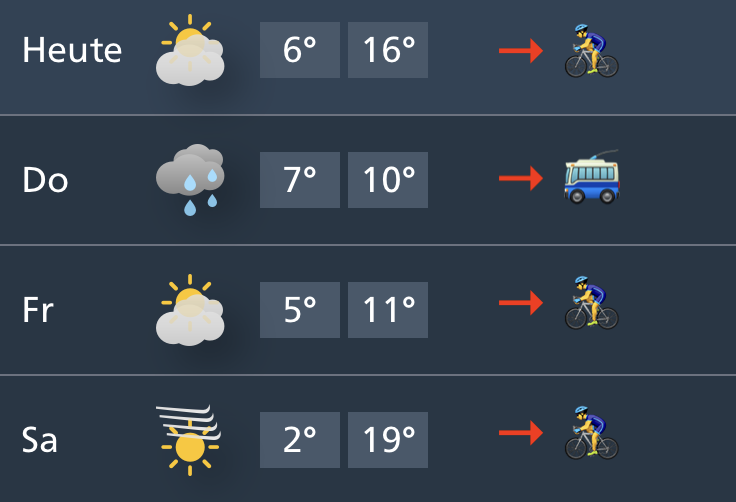
\includegraphics[width=0.7\linewidth]{GrundlagenInfo/00_Programmieren/Figures/if-elif-else-weather}
                  \end{figure}
                  \only<3->{$\rightarrow$ \textcolor{red}{\textbf{und wenn das Velo funktioniert}}}}
        \item<4-> Medizinische Entscheide
              \only<4-5>{\begin{figure}[H]
                      \centering
                      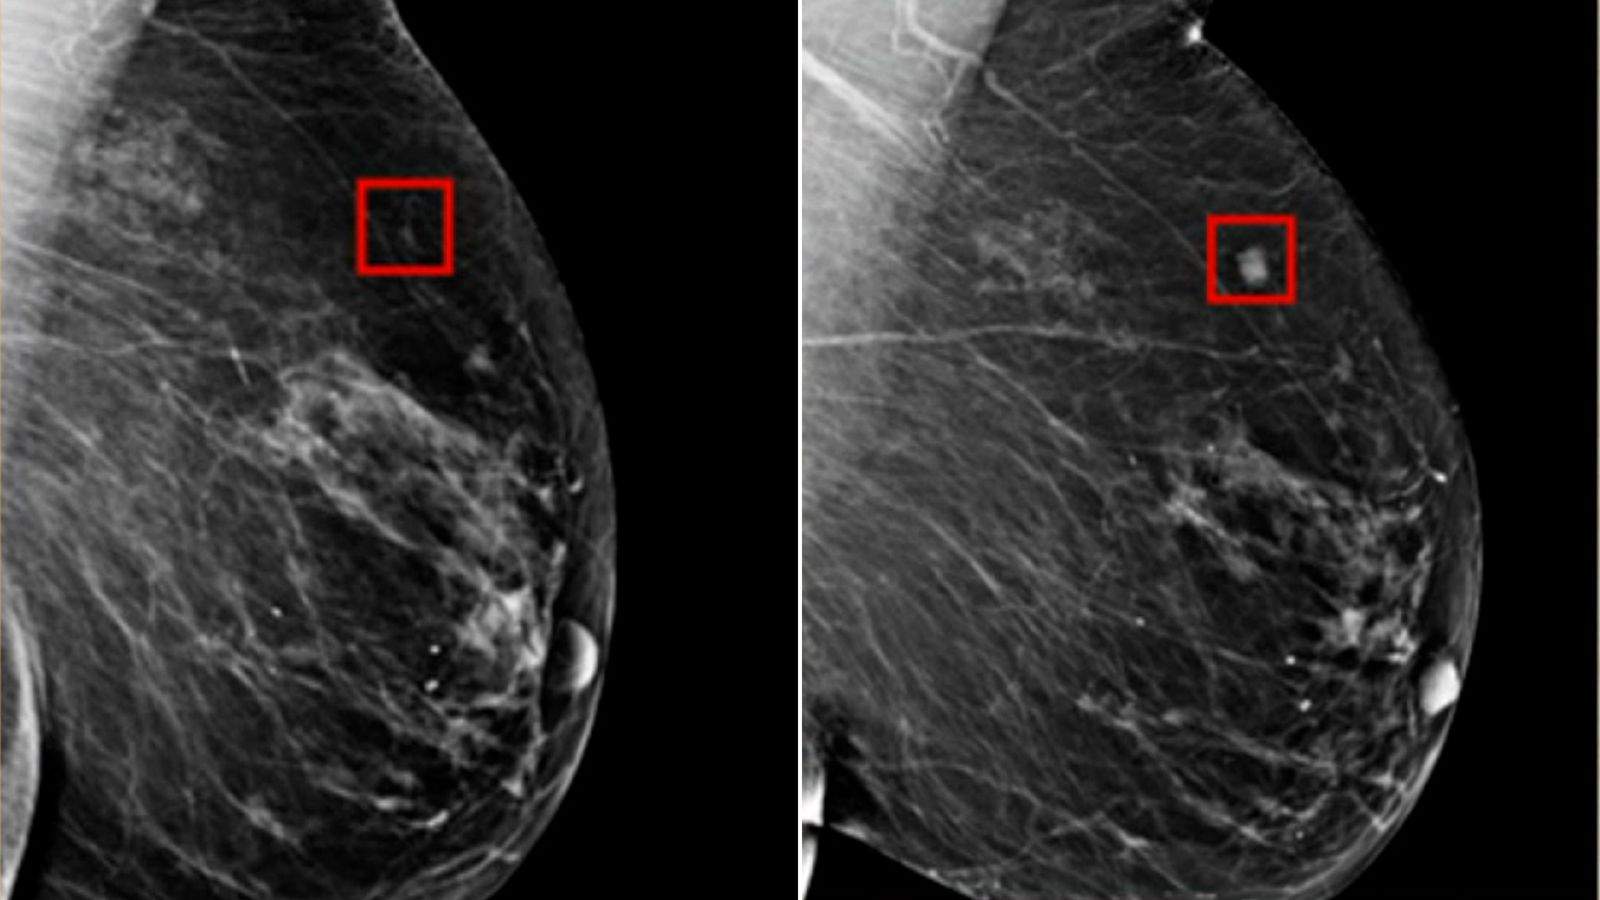
\includegraphics[width=0.7\linewidth]{GrundlagenInfo/00_Programmieren/Figures/if-elif-else-cancer}
                  \end{figure}
                  \only<5->{$\rightarrow$ \textcolor{red}{\textbf{Und wenn die Fachärzte dies bestätigen}}}}
        \item<6-> Etc.
    \end{itemize}
\end{frame}

\begin{frame}[fragile]{Ziele der heutigen Doppel-Lektion}
    Ziele
    \begin{enumerate}[<+->]
        \item \faCheckSquare{} Seine Gedanken \textit{logisch} ausdrücken können
        \item \faCheckSquare{} Mittels Python klare Entscheidungen unter gegebenen Konditionen formulieren können
        \item \faCheckSquare{} Komplexe Konditionen miteinander verbinden
    \end{enumerate}
\end{frame}

\begin{frame}[fragile]{Konditionale Entscheidungen mit Verzweigungen}
    \lstinputlisting[language=Python]{GrundlagenInfo/00_Programmieren/Skript/Code/K04_Logic/ex_if.py}
\end{frame}

\begin{frame}[fragile]{Konditionale Entscheidungen mit Verzweigungen}
    \lstinputlisting[language=Python, basicstyle=\footnotesize\ttfamily]{GrundlagenInfo/00_Programmieren/Skript/Code/K04_Logic/ex_if_else.py}
\end{frame}



\begin{frame}[fragile]{Konditionale Entscheidungen mit Verzweigungen}
    \lstinputlisting[language=Python, basicstyle=\footnotesize\ttfamily]{GrundlagenInfo/00_Programmieren/Skript/Code/K04_Logic/ex_if_elif_else.py}
\end{frame}

\begin{frame}[fragile]{Konditionale Entscheidungen mit Verzweigungen}
    \begin{columns}
        \begin{column}{0.5\textwidth}
            \lstinputlisting[language=Python, basicstyle=\footnotesize\ttfamily]{GrundlagenInfo/00_Programmieren/Skript/Code/K04_Logic/ex_if_elif_else_both.py}
        \end{column}
        \only<2->{
            \begin{column}{0.05\textwidth}
                \centering
                $\Rightarrow$
            \end{column}
            \begin{column}{0.5\textwidth}
                \lstinputlisting[language=Python, basicstyle=\footnotesize\ttfamily]{GrundlagenInfo/00_Programmieren/Skript/Code/K04_Logic/ex_if_elif_else_both_fixed.py}
            \end{column}
        }
    \end{columns}
    \vspace{0.5cm}
    \rule{\textwidth}{.5pt}
    \begin{center}
        Was wird ausgegeben?
    \end{center}
\end{frame}

\begin{frame}[fragile]{Konditionale Entscheidungen mit Verzweigungen}
    \begin{columns}
        \begin{column}{0.54\textwidth}
            \lstinputlisting[language=Python, basicstyle=\footnotesize\ttfamily]{GrundlagenInfo/00_Programmieren/Skript/Code/K04_Logic/ex_if_if_else.py}
        \end{column}
        \only<2->{
            \begin{column}{0.05\textwidth}
                \centering
                $\Rightarrow$
            \end{column}
            \begin{column}{0.54\textwidth}
                \lstinputlisting[language=Python, basicstyle=\footnotesize\ttfamily]{GrundlagenInfo/00_Programmieren/Skript/Code/K04_Logic/ex_if_if_else_fixed.py}
            \end{column}
        }
    \end{columns}


    \vspace{0.5cm}
    \rule{\textwidth}{.5pt}
    \begin{center}
        Was wird ausgegeben?
    \end{center}
\end{frame}


\begin{frame}[fragile]{Mehrere Bedingungen zusammenfassen mit \lstinline|or|}
    \begin{adjustwidth}{-2cm}{-2cm}
        \begin{columns}
            \begin{column}{.46\pagewidth}
                \begin{lstlisting}[escapechar=!, basicstyle=\footnotesize\ttfamily]
k = input("Nenne einen italienischsprachigen Kanton")

if k == "Tessin":
    print("Richtig")
elif k == "Graubünden": 
    print("Richtig")
else:
    print("Falsch")
\end{lstlisting}
            \end{column}
            \begin{column}{.01\pagewidth}
                \rule{0.4pt}{\textheight}
            \end{column}
            \begin{column}{.5\pagewidth}
                Redundanter Code (Gleicher Code mehrfach...)
            \end{column}
        \end{columns}
    \end{adjustwidth}
\end{frame}

\begin{frame}[fragile]{Mehrere Bedingungen zusammenfassen mit \lstinline|or|}
    \begin{adjustwidth}{-2cm}{-2cm}
        \begin{columns}
            \begin{column}{.46\pagewidth}
                \begin{lstlisting}[escapechar=!, basicstyle=\footnotesize\ttfamily]
k = input("Nenne einen italienischsprachigen Kanton")

if k == "Tessin":      !\tikzmark{fromStart}!
    print("Richtig")
elif k == "Graubünden": 
    print("Richtig")   !\tikzmark{fromEnd}!
else:
    print("Falsch")
\end{lstlisting}
            \end{column}
            \begin{column}{.01\pagewidth}
                \rule{0.4pt}{\textheight}
            \end{column}
            \begin{column}{.5\pagewidth}
                    \begin{lstlisting}[escapechar=!, basicstyle=\footnotesize\ttfamily]
            k = input("Nenne einen italienischsprachigen Kanton")
            
            !\tikzmark{toStart}!if k == "Tessin" or k == "Graubünden":
            !\tikzmark{toEnd}!    print("Richtig")
            else:
                print("Falsch")
        \end{lstlisting}
                \only<2->{
                    % annotate listings
                    \begin{tikzpicture}[overlay, remember picture,
                            every edge/.append style = { ->, thick, >=stealth, red!70},
                            every node/.style={draw=red!50,fill=red!50!white,text=black,rounded corners}]
                        \only<2->{
                            \drawBrace{0em}{fromStart}{fromEnd}{}{.5}{}{}
                            \drawBrace{-.5em}{toStart}{toEnd}{}{.5}{mirror}{}
                            % arrow pointing from one code to other
                            \draw[->, style={thick, >=stealth, red!70}] (fromStartfromEnd-coord-arrow) to (toStarttoEnd-coord-arrow);
                        }
                    \end{tikzpicture}
                }
            \end{column}
        \end{columns}
    \end{adjustwidth}
\end{frame}

\begin{frame}[fragile]{Mehrere Bedingungen zusammenfassen mit \lstinline|and|}
    \begin{adjustwidth}{-2cm}{-2cm}
        \begin{columns}
            \begin{column}{.46\pagewidth}
                \begin{lstlisting}[escapechar=!, basicstyle=\footnotesize\ttfamily]
                    temperature = 25 # Aussentemperatur
                    fit = 80 # Fitness
                    if (temperature > 20):   !\tikzmark{fromStart2}!
                        if (fit > 80):
                            print("Fahrrad") !\tikzmark{fromEnd2}!
                \end{lstlisting}
            \end{column}
            \begin{column}{.01\pagewidth}
                \rule{0.4pt}{\textheight}
            \end{column}
            \begin{column}{.5\pagewidth}
                Verschachtelter Code...
            \end{column}
        \end{columns}
    \end{adjustwidth}
\end{frame}

\begin{frame}[fragile]{Mehrere Bedingungen zusammenfassen mit \lstinline|and|}
    \begin{adjustwidth}{-2cm}{-2cm}
        \begin{columns}
            \begin{column}{.46\pagewidth}
                \begin{lstlisting}[escapechar=!, basicstyle=\footnotesize\ttfamily]
                    temperature = 25 # Aussentemperatur
                    fit = 80 # Fitness
                    if (temperature > 20):   !\tikzmark{fromStart2}!
                        if (fit > 80):
                            print("Fahrrad") !\tikzmark{fromEnd2}!
                \end{lstlisting}
            \end{column}
            \begin{column}{.01\pagewidth}
                \rule{0.4pt}{\textheight}
            \end{column}
            \begin{column}{.5\pagewidth}
                    \begin{lstlisting}[escapechar=!, basicstyle=\footnotesize\ttfamily]
                        temperature = 25 # Aussentemperatur
                        fit = 80 # Fitness 
                        !\tikzmark{toStart2}!if (temperature > 20) and (fit > 80):
                        !\tikzmark{toEnd2}!   print("Fahrrad")
        \end{lstlisting}
                \only<2->{
                    % annotate listings
                    \begin{tikzpicture}[overlay, remember picture,
                            every edge/.append style = { ->, thick, >=stealth, red!70},
                            every node/.style={draw=red!50,fill=red!50!white,text=black,rounded corners}]
                        \only<2->{
                            \drawBrace{0em}{fromStart2}{fromEnd2}{}{.5}{}{}
                            \drawBrace{-.5em}{toStart2}{toEnd2}{}{.5}{mirror}{}
                            % arrow pointing from one code to other
                            \draw[->, style={thick, >=stealth, red!70}] (fromStart2fromEnd2-coord-arrow) to (toStart2toEnd2-coord-arrow);
                        }
                    \end{tikzpicture}
                }
            \end{column}
        \end{columns}
    \end{adjustwidth}
\end{frame}

\begin{frame}{Aufgaben}
    Lösen Sie folgende Aufgaben:
    \begin{itemize}
        \item \aufgabebox{5.11 - 5.14} auf Moodle (CodeRunner)
        \item \aufgabebox{5.15} in VS Codium
        \item \challengebox{5.16 - 5.18}
    \end{itemize}
\end{frame}

